\section{From Candidates to Program}

    So far we have only addressed reordering at the Candidate level. In practice, a program can have many Candidates. This is due to the program having several conditional branches and loops. To analyze when we can reordering two events at the program level, we must also address the involvement of conditionals and loops that may be between these two events.
    
    The way we approach this is to not have any assumptions as to why the compiler chooses to do a particular reordering in the program. 
    We instead only check if the reoredered program can have its observable behaviors as a subset of the original. This ensures that the algorithm for the compiler optimization need not change, but that our set of conditions will just be additional checks that can be done before actually doing the reordering. Such an approach makes reordering parametric to the memory model. 

    The downside is that this approach will be conservative as we use no information as to why a particular set of events are reordered. We do not compare and contrast in details the perks of both approaches. This is beyond the scope of this thesis.
    
    \subsection{Addressing programs with Conditionals}

        We first consider programs with conditionals. 
        The following two properties holds for any candidates of programs having conditional branching. 
        \begin{property}{Candidates of Programs with Conditionals}
            \label{CondB1}
            Let $B1$ be the sets of events based on a branch of a conditional in a program $P$. 
            Let $C$ be any Candidate of $P$ and consider $k$ to be a representative event outside the conditional branch. 
            Then $b1 \in B1$ if and only if:
            \begin{align*}
                \exists C \ \text{s.t.} b1 \notin C  
            \end{align*}
            There exists a candidate of the program such that events from the branch cannot be part of it\footnotemark. 
        \end{property}

        \footnotetext{While the property for 1 branch may not always hold (it can be the case that the branch is always taken in any execution) we are defining it for any program. So we assume that every conditional can either be true or false in a program, not just one of them.}

        The above property is general for conditionals, whether it is an ``if-then" (1-branch) clause or ``if-then-else" (2-branch) clause. 
        The latter however, has another property which we define below:
        \begin{property}{Candidates of Programs with Conditionals (2-branch)}
            \label{CondB2}
            Let $B1,B2$ be two sets of events based on each branch of a conditional in a program $P$. 
            Let $C$ be any Candidate of $P$. 
            Then $b1 \in B1 \ \wedge \ b2 \in B2$ if and only if:
            \begin{align*}
                \nexists C \ \text{s.t.} \ b1 \in C \ \wedge \ b2 \in C \\ 
            \end{align*}
            There cannot exist any candidate of the program such that events from both sets can be part of it\footnotemark. 
        \end{property}

        \footnotetext{Note that here we consider every statement in the program unique. So a program like ``if $(c)$ then {$x=1;$} else {$x=1;$}", both the writes to $x$ are unique.}

        Figure~\ref{reord:conditionals} summarizes the two forms of conditionals we can have in any program. 
        \begin{figure}[H]
            \centering 
            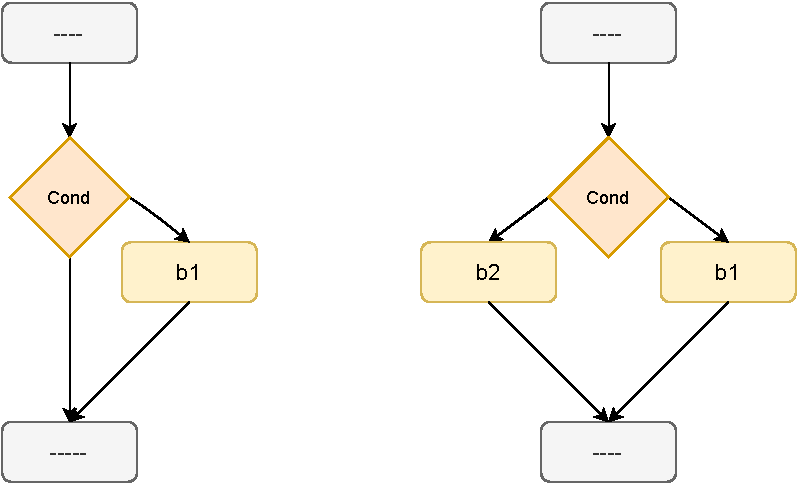
\includegraphics[scale=0.7]{4.InstructionReordering/5.ValidReorderingProgram/Conditionals2Form.pdf}
            \caption{Two forms of conditionals.}
            \label{reord:conditionals}
        \end{figure}


        We use the above two properties to state the following lemma 
        \begin{lemma}
            \label{CondBranchLemma}
            Reordering an statement $e$ inside a conditional to outside a conditional violates Property \ref{CondB1} and Property \ref{CondB2}
        \end{lemma}

        \begin{proof}
            The proof is trivial. 
            By removing a statement outside of a conditional branch, we can get a candidate of a program that would violate both properties. 
        \end{proof}

        The above proof also lets us infer that on reordering an event outside a conditional, there are Candidates that exist with a new event belonging to it. 
        We use this insight to state the following corollary for reordering under conditionals. 
        \begin{corollary}
            \label{ReordCond}
            Consider a program $P$ with conditional branches and its candidates $C_1, C_2, ... , C_n$ in which events $e$ and $d$ present in all of them with $\reln{e}{ao}{d}$. 
            Consider the set of corresponding candidates $C'_1, C'_2, ... , C'_n$ after reordering $e$ and $d$ and its corresponding program $P'$. 
            If the following two conditions hold:
            \begin{gather*}
                Reord(e,d) \ \wedge \ 
                ( \forall C_{i \in [1,n]}, \forall k \in C_i \ \text{s.t.} \ \reln{e}{ao}{k} \wedge \reln{k}{ao}{d}, \    
                Reord(e,k) \wedge Reord(k,d) ). \\
                \nexists C \ s.t. \ 
                    (
                        (e \in C \ \wedge \ d \notin C) \ \vee \ 
                        (e \notin C \ \wedge \ d \in C)
                    ). 
            \end{gather*}
            then the set of observable behaviors of $P'$ is a subset of that of $P$. 
        \end{corollary}

        \begin{proof}

            We prove the second condition first. 
            Assume the second condition does not hold. 
            Then we would have
            \begin{align*}
                \exists C \in P \ s.t. \ 
                (
                    (e \in C \ \wedge \ d \notin C) \ \vee \ 
                    (e \notin C \ \wedge \ d \in C)
                ).
            \end{align*}
            
            By Property \ref{CondB1}, $e$ or $d$ must belong to a conditional branch. 
            If $e$ and $d$ are in different branches of same conditional, then by Property \ref{CondB2} there wouldn't exist any candidate $C$ in $P$ where we could reorder $e$ and $d$. 
            If $e$ and $d$ are of the same conditional branch, and neither one of them belong in any conditional branch nested within, then our above assumption does not hold (simple sequential property of conditional branches).
            
            For the other cases, without loss of generality, let us suppose the first condition holds, i.e. 
            \begin{align*}
                \exists C \in P \ s.t. \ 
                (e \in C \ \wedge \ d \notin C).
            \end{align*}

            The cases for the above can be summarized in the Figure~\ref{reord:cond_branch_cases}: 
            \begin{figure}[H]
                \label{CondCases}
                \centering 
                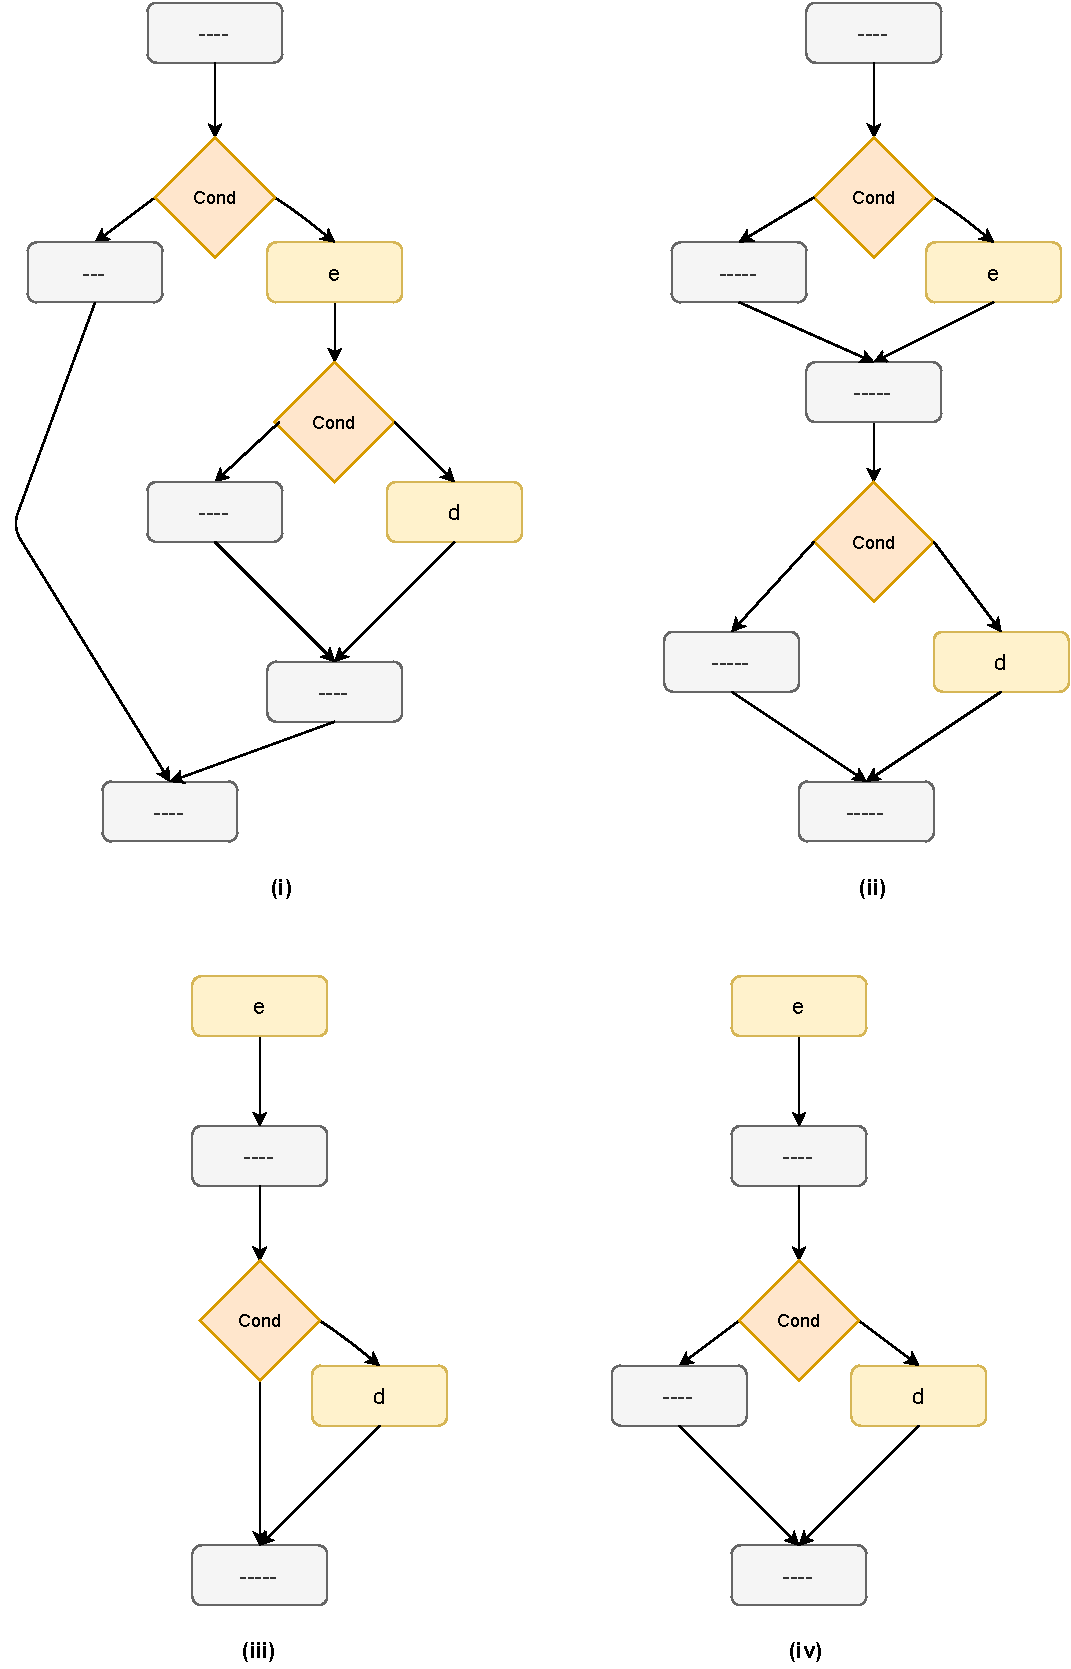
\includegraphics[scale=0.6]{4.InstructionReordering/5.ValidReorderingProgram/ConditionalCases.pdf}
                \caption{Four base cases where $e$ or $d$ are part of some conditional branch.}
                \label{reord:cond_branch_cases}
            \end{figure}

            For cases (i) and (ii), by Lemma \ref{CondBranchLemma}, a new Candidate with event $e$ or $d$ exists without their respective conditional branches being taken.
            For cases (iii) and (iv), by Lemma \ref{CondBranchLemma}, a new Candidate with event $d$ exists without its respective conditional branch being taken.
            Irrespective of $e$ or $d$ being a read or a write, there could be a new $\stck{_{rf}}$ relation be formed with some event $k$ in the Candidate. Thus, we have a new observable behavior\footnotemark. 

            Hence, by contradiction, the second condition must hold.
            
            \footnotetext{Note that this argument is purely in terms of the execution graphs. The new event can possibly have a new reads-from relation established with some event in the graph itself. Since this new node did not exist in the graph before, and since every node in the graph is considered unique, we can infer that a new observable behavior is introduced. Analyzing which such execution graphs are equivalent, would imply drawing equivalence between two different reads-from relations. This could be done as a whole by addressing redundancy introduction optimization. This is not within the scope of the thesis.}

            The first condition holds trivially as it corresponds to Corollary \ref{CorollReord} for each candidate $C_{i\in[1,n]}$. 
            By property of union of sets, we can infer that the set of Observable Behaviors of $P'$ is a subset of that of $P$.

        \end{proof}

  
%------------------------------------------------------------------------------------------------------------------------------------------
    

    \subsection{Addressing Programs with Loops}
        
        Addressing reordering of events in programs with loops is relatively straightforward, leaving one special case. 
        For simplicity (and also without loss of generality), let us consider our program to have only one loop.

        There will be one Candidate for each possible count of loop iteration. 
        For convenience, let us define $C^i$ to be a candidate of program with $i$ iterations of the same loop. 
        Let us also define $e^i$ to be an event within the loop of the program which in a candidate signifies the $i^{th}$ iteration of the corresponding statement. 

        Using the above notation, we define the following corollary for reordering events $e$ and $d$ within a loop.
        The intuition is that if we can reorder $e$ and $d$ in every iteration of the loop, then the observable behaviors of the resultant program is a subset of the original. 
        \begin{corollary}
            Consider a program $P$ with a loop and its candidates $C^1, C^2, ...$ in which events $e$ and $d$ are parts of the loop and present in all of them with $\reln{e}{ao}{d}$. 
            Consider the set of corresponding candidates $C'^1, C'^2, ...$ after reordering $e$ and $d$ in $P$ and its corresponding program $P'$. 
            If the following three conditions hold:
            \begin{gather}
                Reord(e, d) \label{reord:loops1}\\ 
                \forall C^i \in P , \ \forall j \in [1,i], \forall k \ \text{s.t.} \ \reln{e^j}{ao}{k} \wedge \reln{k}{ao}{d^j} \ . \ Reord(e^j, k) \wedge Reord(k, d^j) \label{reord:loops2} \\ 
                \nexists C^i \in P \ s.t. \ 
                    \forall j\!\leq\!i , \ (e^j \in C \ \wedge \ d^j \notin C) \ \vee \ 
                    (e^j \notin C \ \wedge \ d^j \in C) \label{reord:loops3}
            \end{gather}
            then the set of observable behaviors of Program $P'$ is a subset of program $P$.     
        \end{corollary}

        \begin{proof}
        
            The proof for this is fairly straightforward. 
            Condition \ref{reord:loops1} corresponds to Theorem \ref{ThmReord}. 
            Condition \ref{reord:loops2} and \ref{reord:loops3} correspond to Corollary \ref{CorollReord} and \ref{ReordCond} with a slight difference. 
            Because we reorder $e$ and $d$ within a loop, the resultant program's Candidates $C'^i$ will have for each iteration of the loop the events $e$ and $d$ reordered within them. 
            Hence, we need to ensure that reordering is possible in every possible iteration. 
            These conditions precisely define this requirement\footnotemark. 
            
            \footnotetext{Since the compiler cannot practically check for all iterations the set of conditions we have, one might assume that this does not hold in practice. On the contrary, its practical application would just involve checking $Reord(e,k)$ and $Reord(k,d)$ for all such events $k$ that can exist between $e$ and $d$. The reason we did not define it this fashion is because this would need a formal definition of ``between". But this set can be obtained using a straightforward flow-analysis by the compiler. Additionally, Condition \ref{reord:loops3} can always be checked beforehand as it corresponds to checking whether events $e$ and $d$ belong in different conditional branches.}

        \end{proof}

        \paragraph{Reordering Accross Loops}
            What is not so obvious is the case when events are reordered out of the loop. 
            The problem is that we cannot use parent Candidate to generate resultant Candidate of the transformed program. 
            Reordering at the Candidate level does not map directly to Reordering that is done to perform something like Loop invariant code motion. 
            This is because, such a transformation implies introduction/elimination of events in a Candidate.
            We will show in the next chapter that we can in fact define one of its forms, viz. loop invariant code motion using both Reordering and Elimination at the Candidate level.
             
    